\chapter*{Context}
\addcontentsline{toc}{chapter}{Context}

\setlength\epigraphwidth{\textwidth}
\setlength\epigraphrule{0pt}
\epigraph{\justifying\textit{As a technology, microfluidics seems almost too good to be true: it offers so many advantages and so few disadvantages. But it has not yet become widely used. Why not? Why is every biochemistry laboratory not littered with 'labs on chips'? Why does every patient not monitor his or her condition using microfluidic home-test systems? The answers are not yet clear.}}{--- George M. \citeauthor{whitesides2006}, Nature \citeyear{whitesides2006}}

\begin{wrapfigure}{L}{0.50\textwidth}
\centering
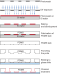
\includegraphics[width=0.45\textwidth]{./ims/mazutis2013.png}
\captionsetup{margin={0pt,6pt},labelfont=bf}
\caption[PDMS soft lithography]{\textbf{\acrshort{pdms} soft lithography.} Taken from \cite{mazutis2013}}
\label{fig:mazutis2013}
\vspace{-20pt}
\end{wrapfigure}

In \citeyear{whitesides2006}, when \acrshort{pdms} was still a rare sight in most labs, George M. Whitesides pondered why the seemingly inconspicuous polymer had not yet revolutionised molecular research. It had been eight years since the many benefits of \acrshort{pdms} soft lithography and its possible applications in microfluidics were originally proposed \citep{xia1998}. Today, more than a decade after Whitesides' \citeyear{whitesides2006} Nature Insight article, soft elastomer lithography has become the most widespread technique for microfluidic device manufacturing and the \citeyear{xia1998} paper has been cited more than 11 000 times. The technique has found many applications in various branches of science. In biotechnology, where its low toxicity, inherent hydrophobicity, transparency and inert nature pose many advantages, \acrshort{pdms} soft lithography has become a staple technique. Droplet microfluidics, a subset of microfluidics where pico- to nanolitre droplets are produced by focusing two immiscible phases, has been used extensively in bioscience in the past years. The ultra-low volumes associated with droplet microfluidics reduce reagent usage, leading to a reduction in overall cost, and can in some cases increase reaction efficiency \citep{wu2014}. The technology has been used in a wide array of biological applications: as a platform for high-throughput drug screening assays \citep{brouzes2009}, in the analysis of protein expression of single cells \citep{huebner2007} and even in the engineering of stem cell growth niches \citep{allazetta2015}.\pms

\begin{wrapfigure}{L}{\textwidth/2}
\centering
\includegraphics[width=\textwidth/2]{./ims/davie.png}
\captionsetup{margin={6pt,6pt},labelfont=bf}
\caption[Single-cell atlas of Drosophila brain]{\textbf{Single-cell atlas of Drosophila brain.} Transcriptomes of 57k single cells are sequenced and computationally separated to discern different cell types. \citep{davie2018}}
\label{fig:davie2018}
\vspace{-20pt}
\end{wrapfigure}

In the past few years, droplet microfluidics have also been applied in single-cell technology. Single cells are co-encapsulated into nanolitre droplets together with various reagents and barcoded hydrogel beads in order to capture their \acrshort{mrna} content, which is then molecularly barcoded. Due to the barcoding process, \acrshort{mrna} from single cells can be sequenced together and computationally separated. An example of such an application is given in figure \ref{fig:davie2018}. Here, 57 000 fly brain cells were processed using droplet-microfluidic single-cell technology, and computationally analysed to form a comprehensive atlas of the different cell types present in the Drosophila brain.\pms

This thesis revolves around optimisation and innovation in the technical/molecular side of the single-cell analysis field. The work can be split in two main lines: the first line (chapter \ref{ch:indrop}) focuses on the implementation and optimisation of inDrop, a pre-existing droplet-microfluidic \acrlong{scrna-seq} platform \citep{klein2015, zilionis2017}. In the second line (chapter \ref{ch:dropatac}), the droplet microfluidics and molecular engineering expertise acquired in the first part is applied to develop an entirely new protocol. Here, we attempt to prototype a microfluidic approach for \acrshort{atac-seq} ("Drop-\acrshort{atac}"), which as of today only exists as a commercial package. As both the optimised inDrop and Drop-\acrshort{atac} are situated on the far end of the throughput scale, they pose high potential in screening assays where large numbers of cells need to be analysed rapidly.\pms

The end-goal is to explore the new possibilities posed by combining droplet microfluidics and modern molecular cell-analysis. This combination has only recently emerged as a powerful tool in (systems) biology, but is already revolutionising the field. As the droplet-microfluidic single-cell techniques are only in their infancy, there is still a lot of room for improvement and innovation, an opportunity we address in this work.\pms
